\documentclass{article}
\usepackage{amsmath}
\usepackage{amssymb}
\usepackage{graphicx}
\usepackage{hyperref}
\usepackage[version=4]{mhchem}

\title{Problem 16}
\date{}

\begin{document}
\maketitle

\section*{Problem}
As shown in the figure, in triangle \(A B C, M\) is the midpoint of \(B C\). \(A N=\frac{1}{3} A C\). Connect \(B N\) and denote the point where \(B N\) meets \(A M\) to be \(P\). Show that \(B P=3 P N\).\\
\centering
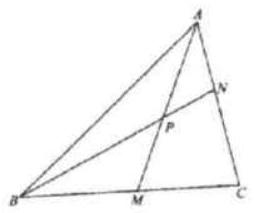
\includegraphics[width=\textwidth]{images/129(4).jpg}

\section*{Solution}
This problem is the same as Example 4. Here, we show two new, different ways to solve it.


Method 1:\\
Draw a line through \(N\) parallel to \(A M\) to meet \(C M\) at \(D\).\\
Since \(\frac{A N}{A C}=\frac{1}{3}, \frac{M D}{M C}=\frac{1}{3}\).\\
\centering
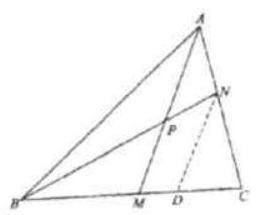
\includegraphics[width=\textwidth]{images/139.jpg}

We know that \(B M=M C\), so \(\frac{M D}{B M}=\frac{1}{3}\).\\
We also know that \(M P / / D N\), so \(\frac{P N}{B P}=\frac{1}{3}\)\\
\(\Rightarrow \quad B P=3 P N\).\\
Method 2:\\
Draw a line through \(N\) parallel to \(B C\) to meet \(A M\) at \(D\).\\
\centering
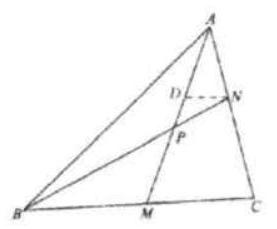
\includegraphics[width=\textwidth]{images/139(2).jpg}

Since \(\triangle A D N \sim \triangle A M C, \frac{A N}{A C}=\frac{1}{3}\).\\
Since \(M B=M C, 3 D N=M C=M B\).\\
Since \(\triangle P D N \sim \triangle P M A, \frac{D N}{M C}=\frac{P N}{P B}=\frac{1}{3}\)\\
\(\Rightarrow \quad B P=3 P N\).

\end{document}
